% ---------------------------------------------------------------------------
% Hierbei handelt es sich um eine angepasste Vorlage von Stefan Macke
% Permalink zur originellen Vorlage: http://fiae.link/LaTeXVorlageFIAE
% ---------------------------------------------------------------------------
\documentclass[
	ngerman,
	toc=listof, % Abbildungsverzeichnis sowie Tabellenverzeichnis in das Inhaltsverzeichnis aufnehmen
	toc=bibliography, % Literaturverzeichnis in das Inhaltsverzeichnis aufnehmen
	footnotes=multiple, % Trennen von direkt aufeinander folgenden Fußnoten
	parskip=half, % vertikalen Abstand zwischen Absätzen verwenden anstatt horizontale Einrückung von Folgeabsätzen
	numbers=noendperiod % Den letzten Punkt nach einer Nummerierung entfernen (nach DIN 5008)
]{scrartcl}
\usepackage[utf8]{inputenc} % muss als erstes eingebunden werden, da Meta/Packages ggfs. Sonderzeichen enthalten

%\newcommand{\titel}{UI5 App: Abwesenheitskalender}
%\newcommand{\untertitel}{Erweiterung der Mitarbeiterverwaltungplatform}
\newcommand{\titel}{Fiori App: Abwesenheitskalender }
\newcommand{\untertitel}{Integration der Abwesenheitsübersicht in das "MIBS virtualDesk" }

\newcommand{\kompletterTitel}{\titel{} -- \untertitel}

\newcommand{\autorName}{Tom Porten}
\newcommand{\autorAnschrift}{Lohbecker Berg 30}
\newcommand{\autorOrt}{45470 Mülheim an der Ruhr}
\newcommand{\identnummer}{122874724-92}

\newcommand{\betriebLogo}{MIBSlogo.png}
\newcommand{\betriebName}{MIBS AG}
\newcommand{\betriebAnschrift}{Wasserstraße 3-7}
\newcommand{\betriebOrt}{45468 Mülheim an der Ruhr}

\newcommand{\ausbildungsberuf}{Fachinformatiker für Anwendungsentwicklung}
\newcommand{\betreff}{Dokumentation zur betrieblichen Projektarbeit}
\newcommand{\pruefungstermin}{Winter 2024}
\newcommand{\abgabeTermin}{21.11.2024}
 % Metadaten zu diesem Dokument (Autor usw.)
\input{Sonstiges/Packages} % verwendete Packages
\input{Sonstiges/Stil} % Definitionen zum Aussehen der Seiten
\input{Sonstiges/Befehle} % eigene allgemeine Befehle, die z.B. die Arbeit mit LaTeX erleichtern

\begin{document}
% ---------------------------------------------------------------------------
% Deckblatt
\phantomsection
\thispagestyle{plain}
\pdfbookmark[1]{Deckblatt}{deckblatt}
\begin{titlepage}

\begin{center}

\includegraphics[scale=0.2]{ihk.jpg}\\[1ex]
\Large{Abschlussprüfung \pruefungstermin}\\[3ex]

\Large{\ausbildungsberuf}\\
\LARGE{\betreff}\\[4ex]

\huge{\textbf{\titel}}\\[1.5ex]
\Large{\textbf{\untertitel}}\\[4ex]

\normalsize
Abgabetermin: \abgabeTermin\\[3em]
\textbf{Prüfungsbewerber:}\\
\autorName\\
\autorAnschrift\\
\autorOrt\\[2ex]
\textbf{Identnummer:}\\
\identnummer\\[5ex]

\includegraphics[scale=0.09]{\betriebLogo}\\[2ex]
\textbf{Ausbildungsbetrieb:}\\
\betriebName\\
\betriebAnschrift\\
\betriebOrt\\[5em]
\end{center}

\end{titlepage}
\cleardoublepage

% ---------------------------------------------------------------------------
% Inhaltsverzeichnis & co.
\phantomsection
\pagenumbering{Roman}
\pdfbookmark[1]{Inhaltsverzeichnis}{inhalt}
\tableofcontents

\cleardoublepage

\phantomsection
\listoffigures
\cleardoublepage

\phantomsection
\listoftables
\cleardoublepage

\phantomsection
\lstlistoflistings
\cleardoublepage

%\newcommand{\abkvz}{Abkürzungsverzeichnis}
%\renewcommand{\nomname}{\abkvz}
%\section*{\abkvz}
%\markboth{\abkvz}{\abkvz}
%\addcontentsline{toc}{section}{\abkvz}
%\input{Abkuerzungen}
%\clearpage

% ---------------------------------------------------------------------------
% Kapitel

\pagenumbering{arabic}

\section{Einleitung}
\label{sec:Einleitung}
Die folgende Projektdokumentation beschreibt den Ablauf des IHK-Abschlussprojektes, das im Rahmen der Ausbildung zum Fachinformatiker Fachrichtung Anwendungsentwicklung durchgeführt wurde. Der Ausbildungsbetrieb ist die MIBS AG, ein SAP-Beratungsunternehmen mit Sitz in Mülheim an der Ruhr. Zurzeit beschäftigt die MIBS AG rund 94 Mitarbeiter\footnote{Stand November 2024}. Das Unternehmen bietet SAP-Beratung und Projektmanagement an und vertreibt außerdem sein eigenes Produkt „SMART“, ein Testwerkzeug für SAP-Anwendungen.
Darüber hinaus entwickelt die MIBS AG ihr eigenes HCM-Tool\footnote{Software die Unternehmen bei der Verwaltung, Planung und Optimierung ihrer Personalressourcen unterstützt} namens \textbf{MIBS virtualDesk}. Dieses wird für die Organisation interner Prozesse, wie beispielsweise Urlaubsanträge, Krankmeldungen oder Zeitnachweise, genutzt.

\subsection{Projektbeschreibung}
\label{sec:Projektbeschreibung}
Derzeit werden im Backoffice der MIBS AG verschiedene operative Aufgaben manuell bearbeitet und in Excel-Tabellen dokumentiert. Hierzu gehören unter anderem das Übertragen von Abwesenheiten von Mitarbeitern aus dem MIBS virtualDesk sowie die Freigabe von Urlaubsanträgen nach deren Erfassung in der Excel-Datei.  
Dieses Dokument wird außerdem regelmäßig zur Planung interner Projekte und Schulungen verwendet. Auch für das Abgleichen von Verfügbarkeiten der Mitarbeiter durch Vorstand oder Teamleiter kommt dieses Dokument zum Einsatz.
In diesem Projekt soll sowohl der gerade beschriebene Prozess vereinfacht werden als auch die manuelle Pflege der Excel-Datei entfallen.


\subsection{Projektziel}
\label{sec:Projektziel}
Das Ziel des Projektes ist das Ersetzen der Excel-Datei durch eine Webanwendung innerhalb des MIBS virtualDesk der MIBS AG.
Folglich soll hierdurch der paralelle Pflegeaufwand entfallen.
Die Angestelltendaten sollen über das bestehende SAP-System verarbeitet werden.
Mitarbeiterabwesenheiten sollen aggregiert und über eine App innerhalb des MIBS virtualDesk verfügbar gemacht werden. Die Abwesenheitszeiträume sollen in einem Kalender, in dem jeder Mitarbeiter aufgelistet ist, ausgegeben werden. Des Weiteren sollen Funktionen für die Filterung der Mitarbeiter bereitgestellt werden.
Unter den angezeigten Daten sollen die Urlaubs- und Krankheitstage, sowie deren aktueller Status angezeigt werden. Zusätzlich sollen die Schulblöcke der Azubis ausgegeben werden.

\subsection{Projektumfeld}
\label{sec:Projektumfeld}
Auftraggeber des Projektes ist der Vorstand der MIBS AG, vertreten durch Marcel Ebert. Betreut wird das Projekt von der Abteilungsleitung des „MIBS Technology Hub“. Der zuständige Ansprechpartner ist Rafael Kopytto. Das Projekt ist für den Zeitraum 15.10.2024 – 21.11.2024 terminiert.

Die Abteilung MTH beobachtet und bewertet neue SAP Entwicklungstrends und unterstützt deren Kunden in der Implementierung dieser. Weiterhin betreut sie die Entwicklung und Wartung des MIBS virtualDesk.


Hierbei wurde sich auf die Entwicklung von RESTful-Anwendungen sowie darauf basierenden Webanwendungen spezialisiert. Primär kommen dabei ABAP RAP\footnote{\label{RAP}RESTful Application Programming – Modell von SAP zur Entwicklung cloudfähiger Anwendungen} für das Backend sowie SAPUI5\footnote{\label{fn:UI5}JavaScript-Framework von SAP zur Entwicklung responsiver Webanwendungen}, insbesondere das Framework Fiori Elements, für das Frontend zum Einsatz. 


\subsection{Projektbegründung}
\label{sec:Projektbegründung}
Die MIBS AG versucht fortlaufend ihre internen Prozesse zu optimieren. Besonders im Bereich des Backoffice wird versucht, manuelle und redundante Aufgaben zu automatisieren und umzustrukturieren. Der gesamte Prozess der Abwesenheitspflege erfordert einen kontinuierlichen manuellen Aufwand und beinhaltet ebenfalls eine redundante Datenpflege. Zum einen werden die Abwesenheiten der Mitarbeiterdaten täglich händisch in der Excel-Tabelle aktualisiert, welches einen wiederkehrenden Aufwand für das Backoffice bedeutet. Zum anderen besteht eine hohe Fehleranfälligkeit bei dem Übertragen der Daten.
Diese Umstände führten zu der Entscheidung, die Abwesenheitsübersicht als App im MIBS virtualDesk zu integrieren.

\subsection{Projektabgrenzung}
\label{sec:Projektabgrenzung}
Das Projekt ist so strukturiert, dass es ausschließlich als Datenanzeige fungiert. Die Hauptfunktion besteht darin, Informationen bereitzustellen, die aus einer definierten Datenquelle abgerufen werden. Es ist ausdrücklich festgelegt, dass die Anwendung keine Funktionen zur Änderung, Löschung oder Neuanlage von Daten bereitstellt. Die zugrunde liegenden Daten bleiben unverändert.


\section{Projektvorgehen}
\label{sec:Projektvorgehen}

\subsection{Planungsphase}
\label{sec:Planungsphase}
Die Umsetzung des Projektes umfasst insgesamt 80 Arbeitsstunden. Diese wurden im Vorfeld in verschiedene Phasen aufgeteilt, die während der Projektentwicklung durchlaufen werden. Eine grobe Übersicht der Zeitplanung sowie die Hauptphasen können der \TabelleRef{tab:GroberZeitplan} entnommen werden. % Frage: Zeitform - werden oder wurden?
Diese Hauptphasen lassen sich in kleinere Arbeitsschritte unterteilen, um den Fortschritt und die Aufgabenverteilung genauer darzustellen. Eine detaillierte Übersicht der einzelnen Phasen wird im \Anhang{app:Zeitplanung} aufgeschlüsselt.

\tabelle{Grober Zeitplan}{tab:GroberZeitplan}{GroberZeitplan}

\subsection{Ressourcenplanung}
\label{sec:Ressourcenplanung}
Die Auswahl der verwendeten Software erfolgte unter der Maßgabe, auf bereits lizenzierte oder frei verfügbare (Open Source) Software zurückzugreifen, um die Projektkosten zu minimieren. Eine detaillierte Auflistung der eingesetzten Tools und Ressourcen befindet sich im \Anhang{app:Ressourcen}.

\subsection{Entwicklungsprozess}
\label{sec:Entwicklungsprozess}
Im Rahmen dieses Projektes wurde das erweiterte Wasserfallmodell gewählt. Dieses bietet eine klar strukturierte und sequenzielle Vorgehensweise, die den Anforderungen und der Komplexität dieses Projektes optimal entspricht. 
Das erweiterte Wasserfallmodell basiert auf dem klassischen Wasserfall-modell, welches durch seine Phasenstruktur – \textbf{Anforderungsanalyse}, \textbf{Design}, \textbf{Implementierung}, \textbf{Test} und \textbf{Wartung} – einen linearen Projektablauf gewährleistet. Darüber hinaus bietet das erweiterte Modell die Flexibilität, frühere Phasen zu revidieren und Anpassungen vorzunehmen, falls während der Entwicklung unerwartete Änderungen oder Erkenntnisse auftreten. Diese erweiterte Version erlaubt somit gezielte Rücksprünge in frühere Phasen, ohne die gesamte Prozesskette zu unterbrechen. Dies verringert die Risiken, die durch Fehlspezifikationen oder unvorhergesehene Anforderungen entstehen könnten.
% Quelle notwendig?
\section{Analysen}
\label{sec:Analysen}

\subsection{Ist-Analyse}
\label{sec:Ist-Analyse}
%in den verschiedenen Status (Planung, Antrag, genehmigt), welche ebenfalls halber Urlaubstage und Sonderurlaub beinhalten 
Derzeit verwaltet unser Backoffice für jeden Mitarbeiter alle Krankheitstage, Urlaubsanträge sowie Schulblöcke der Auszubildenden in einem tagesgenauen Excel-Dokument. Die Urlaubsanträge, welche ebenfalls halbe Urlaubstage und Sonderurlaub beinhalten, werden mit den verschiedenen Status (Planung, Antrag, genehmigt) eingetragen.
Das Dokument wird verwendet, um Schulungen oder Projekte zu planen, Urlaubszeiträume abzustimmen und um gegenüber dem Vorstand stets aussagefähig zu sein, wenn dieser Fragen zu Abwesenheiten hat. 

Für die Verwaltung interner Angelegenheiten wird das MIBS virtualDesk verwendet. Die Plattform besteht aus einer SAPUI5/Fiori Elements\footnote{\label{Fiori}SAP Framework für UI5-basierte Anwendungen} Web-Oberfläche und einem SAP S/4HANA\footnote{ERP-Suite basierend auf der In-Memory-Datenbank HANA} Backend. Dieses verfügt über Apps, mit welchen unter anderem Urlaubsanträge und Krankmeldungen gepflegt werden können. Auch die Zeiträume der Schulblöcke für die Auszubildenden werden bereits von der Ausbildungsleitung im MIBS virtualDesk gepflegt. Die Informationen aus diesen Apps werden genutzt, um die Excel-Datei täglich zu aktualisieren. Dazu müssen die verschiedenen Apps des MIBS virtualDesk aufgerufen und die Informationen manuell in das Dokument übertragen werden. Gleichzeitig wird die Tabelle neben dem MIBS virtualDesk geöffnet, um während der Bearbeitung einen Überblick über mögliche Terminüberschneidungen zu erhalten. Die Liste wird gleichzeitig von der Ausbildungsleitung genutzt, um anstehende Ausbildungsinhalte zu planen. Die tägliche Pflege und der Abgleich beansprucht wertvolle Zeit des Backoffice-Teams.
% beansprucht oder beanspruchen?
% TODO Vorschlag überprüfen
% Die MIBS AG verwendet für ihre internen, administrativen und mitarbeiterbezogenen Prozesse eine browserbasierte Plattform, das sogenannte MIBS virtualdesk (kurz MVD). Das MVD besteht aus einer SAPUI5/Fiori Web-Oberfläche und einem SAP S/4HANA Backend. Es verfügt über Apps, in denen Mitarbeiter- und Kundendaten hinterlegt, Kundeneinsätze und -projekte dokumentiert sowie Arbeitszeiten und sämtliche An- und Abwesenheiten (Krankheit, Urlaub, Sonderurlaub, Berufsschule) erfasst werden. 
% Es gibt allerdings keine App, die die An- und Abwesenheitsdaten der Mitarbeiter übersichtlich zusammenfasst und anzeigt, so dass das Backoffice gezwungen ist, eine Excel-Tabelle zu führen, in die diese Daten täglich manuell aus dem MVD übertragen werden. Hierzu müssen nacheinander die jeweiligen Apps (Urlaub, Krankheit) geöffnet und die tagesaktuellen Daten pro Mitarbeiter in die Exceltabelle übertragen werden. Die tägliche Pflege und der Abgleich beansprucht wertvolle Zeit des Backoffice-Teams.


\subsection{Wirtschaftlichkeitsanalyse}
\label{sec:Wirtschaftlichkeitsanalyse}

\subsubsection{\gqq{Make-or-Buy} Entscheidung}
\label{sec:Make-or-Buy Entscheidung}
Bei der im Betrieb verwendeten Software, dem MIBS virutalDesk, handelt es sich um eine eigens entwickelte Individualsoftware. Der Markt bietet hierfür keine passende Lösung, die alle Anforderungen erfüllt. Aus diesem Grund soll das Projekt als interne Entwicklung realisiert werden.

\subsubsection{Projektkosten}
\label{sec:Projektkosten}

Im Folgenden wurden die voraussichtlich anfallenden Kosten kalkuliert. Die Projektkosten setzen sich aus den Personalkosten und dem Gemeinkostenzuschlag zusammen. 
Die Personalkosten sind folglich aufgeteilt: Auf den Auszubildenden, welcher für die Umsetzung des Projektes zuständig ist, den Projektbetreuer, der das Codereview durchführt und das Projekt beratend betreut sowie die Bürofachkraft des Backoffice, welche in die Anwendung eingearbeitet werden muss.
Bei den Gehältern handelt es sich um Mittelwerte, die von der Personalabteilung bereitgestellt worden sind. Über den Gemeinkostenzuschlag werden alle Kosten erfasst, die nicht spezifisch zuzuordnen sind. Unter diese fallen beispielsweise Strom- oder Verwaltungskosten.
%TODO fußnote Fakura - sowas wie: Arbeitszeit, die unmittelbar an einem Kundenprojekt aufgewendet wird

\tabelle{Kostenrechnung}{tab:Kostenrechnung}{Kostenrechnung}
\newpage

\subsubsection{Amortisationsdauer}
\label{sec:Amortisationsdauer}

Bevor die Amortisationsdauer berechnet werden kann, muss zunächst der aktuelle Zeitaufwand ermittelt werden. Hierfür wurde über die Dauer einer Arbeitswoche die Höhe des Zeitaufwands dokumentiert. In der Erfassung wurde ausschließlich die Pflege der Daten berücksichtigt, da dieser Arbeitsschritt komplett entfallen soll. Wie aus \TabelleRef{tab:Wöchentlicher Pflegeaufwand} zu entnehmen ist, beträgt der durchschnittliche, wöchentliche Aufwand zum Pflegen der Daten 15 Minuten pro Tag.

\tabelle{Wöchentlicher Pflegeaufwand}{tab:Wöchentlicher Pflegeaufwand}{Wöchentlicher Pflegeaufwand} 
% Fußnote Gemeinkostenzuschlag

Für die Ermittlung der Amortisationsdauer, wird zunächst die jährliche Einsparung berechnet. Diese ergibt sich aus dem jährlichen Arbeitsaufwand sowie den Personalkosten. Der jährliche Aufwand definiert sich durch die Arbeitstage multipliziert mit dem täglichen Aufwand. Die jährlichen Arbeitstage belaufen sich nach Abzug der Betriebsferien auf 246 Tage\footnote{Arbeitstage in der MIBS AG für 2024}.

\[
0{,}25 \, \frac{\text{Stunde}}{\text{Tag}} \times 50 \, \frac{\text{€}}{\text{Stunde}} \times 246 \, \frac{\text{Tage}}{\text{Jahr}} = 3075 \, \frac{\text{€}}{\text{Jahr}}
\]

% TODO ggf. auf nächste Seite
Die Amortisationsdauer ergibt sich wie folgt:

\[
\text{Amortisationsdauer} = \frac{\text{Projektkosten}}{\text{Jährliche Einsparung}}
\]

\[
\frac{3245\,\text{€}}{3075\,\text{€/Jahr}} \approx 1{,}055 \, \text{Jahre}
\]
Wie in \Abbildung{Amortisationsdauer} ersichtlich, zeigt sich, dass sich das Projekt nach etwa 1,055 Jahren beziehungsweise rund 12,7 Monaten refinanziert.


\begin{figure}[htb]
\centering
\includegraphicsKeepAspectRatio{Amortisationsdauer.png}{0.7}
\caption{Amortisationsdauer}
\label{fig:Amortisationsdauer}
\end{figure}

\subsubsection{Nicht monetäre Vorteile}
\label{sec:Nicht monetäre Vorteile}
Neben den kalkulierbaren Kostenersparnissen ergeben sich durch dieses Projekt auch nicht monetarisierbare Vorteile. Durch das gezielte Wegfallen von redundanten Aufgaben, beispielsweise der täglichen Datenpflege, kann mit einer Steigerung der Arbeitsmoral gerechnet werden. 
Des Weiteren wird das Risiko der Übertragung fehlerhafter Daten ausgeschlossen. 
Nicht zuletzt trägt es zu der Digitalisierung, Modernisierung und Vereinheitlichung der internen Prozesse im Unternehmen über das MIBS virtualDesk bei.


\subsection{Risikoanalyse}
\label{sec:Risikoanalyse}
Vor Projektbeginn wurde eine Risikomatrix gemäß ISO 31010 erstellt, um die potenziellen Risiken zu bewerten. Die X-Achse zeigt die Schwere der Folgen, die Y-Achse die Eintrittswahrscheinlichkeit. Risiken im \textcolor{Green}{grünen} Bereich gelten als unkritisch, während \textcolor{Goldenrod}{gelbe} Risiken Anpassungen in der Planung erfordern. Risiken im \textcolor{red}{roten} Bereich stellen eine erhebliche Gefährdung des Projektplans dar und erfordern ein gezieltes Risikomanagement. Die Matrix dient als Grundlage für die Risikobewertung durch die Projektverantwortlichen.\\ 
\newpage
Als plausible Risiken werden erkannt:
\begin{enumerate}
\item \textbf{Krankheit des Entwicklers:\\}
Da die Entwicklung von einem einzelnen Entwickler durchgeführt wird, kann ein krankheitsbedingter Ausfall kritisch sein. Der geplante Aufwand enthält jedoch Puffer, um Verzögerungen durch intensivere Arbeit an anderen Projekttagen auszugleichen. Aufgrund vergangener Erfahrungen, wird dieses Risiko als gering eingestuft. Eine lückenlose Dokumentation aller Prozesse und Entwicklungsschritte stellt sicher, dass bei längerer Abwesenheit des Entwicklers eine reibungslose Übergabe möglich ist.
\item \textbf{Ausfall der Hardware:\\}
Ein Ausfall der Hardware wird, basierend auf Erfahrungswerten, als unwahrscheinlich eingestuft. Im Falle eines Ausfalls stehen Ersatzgeräte der MIBS AG zur Verfügung, um Verzögerungen zu vermeiden.
\item \textbf{SAP-Systemausfall:\\}
Der Ausfall des SAP-Systems hätte erhebliche Auswirkungen, da das Backend vollständig auf diesem System basiert. Dieses Risiko wird jedoch als unwahrscheinlich eingeschätzt. Teile des Frontends können unabhängig vom System lokal entwickelt werden, wodurch die Auswirkungen begrenzt werden.
\item \textbf{Ausfall des Fachbereiches:\\}
Ein vollständiger Ausfall des Fachbereichs wird aufgrund der personellen Besetzung als unwahrscheinlich betrachtet. Die Auswirkungen wären gering, da die Anforderungen bereits definiert und die fachlichen Prozesse durchdacht sind.
\end{enumerate}

\begin{figure}[htb]
\centering
\includegraphicsKeepAspectRatio{Risiko.png}{0.9}
\caption{Risikoanalyse}
\label{fig:Risikoanalyse}
\end{figure}

\subsection{Datenanalyse}
\label{sec:Datenanalyse}
Für die Datenanalyse wurde das bestehende Datenmodel untersucht. Dabei wurden die benötigten Views identifiziert.
Eine Beschreibung der Views sowie deren Zusammenspiel wird im \Anhang{app:Datenanalyse} genauer erläutert.

%TODO: Tag statt Periode erwähnen? Bzw Daten hier beschreiben
\newpage
\section{Entwurfsphase}
\label{sec:Entwurfsphase}

\subsection{Architekturdesign}
\label{sec:Architekturdesign}
\begin{wrapfigure}{r}{0.5\textwidth} % r = rechts, Breite = 50% der Textbreite
    \centering
    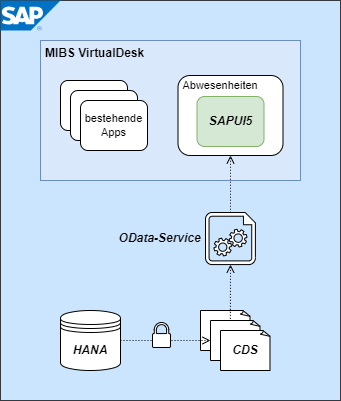
\includegraphics[width=\linewidth, keepaspectratio]{Bilder/Komponenten.png} % Bild einfügen
    \caption{Komponenten}
    \label{fig:Komponenten}
\end{wrapfigure}

Das Architekturdesign der Anwendung basiert auf einer modularen Struktur, bei der verschiedene Komponenten zusammenarbeiten. Dies soll die Wiederverwendbarkeit und Wartbarkeit der einzelnen Komponenten erhöhen. 
Die Anwendung wird als SAP Fiori App innerhalb des MIBS VirtualDesk, welches auf einem SAP Fiori Launchpad basiert, veröffentlicht. Das Frontend wird, mithilfe des SAP Fiori Frameworks, als „Fiori Freestyle“-App\footnote{Entwicklungsansatz für individuell entwickelte SAP Fiori-Anwendung ohne Vorlagen} implementiert. Dieses erfordert einen höheren Entwicklungsaufwand, bietet dafür jedoch eine bessere Erweiterbarkeit der Benutzeroberfläche.

Der OData-Service\footnote{Open Data Protocol - standardisiertes Protokoll für Zugriff auf Daten über das Web} stellt das zentrale Bindeglied zwischen dem Frontend und der Datenquelle dar. Er ermöglicht den selektiven Zugriff auf die relevanten Abwesenheitsdaten der Mitarbeiter. Die Daten, die durch diesen Service abgerufen werden, basieren auf Core Data Services (CDS) Views, die in SAP S/4HANA definiert sind. Diese CDS Views werden mit dem SAP-Berechtigungssystem verknüpft, sodass nur autorisierte Benutzer Zugriff auf die entsprechenden Informationen haben.

%-	Entwickung + Tests auf dev system?

Insgesamt ermöglicht dieses Design eine sichere, performante und benutzerfreundliche Darstellung der Abwesenheitsinformationen, die in Echtzeit im Fiori Launchpad bereitgestellt werden. Das Zusammenspiel aus SAPUI5-Frontend, OData-Service und CDS Views stellt sicher, dass die Anwendung sowohl flexibel als auch an die speziellen Anforderungen der MIBS AG angepasst ist.

\subsection{UI Design}
\label{sec:UI Design}
Das User Interface (UI) wird mit Hilfe des SAP Fiori Frameworks so gestaltet, dass es eine intuitive Kalenderübersicht der Mitarbeiter-Abwesenheiten der MIBS bietet. Der Kalender wird den zentralen Bestandteil der Oberfläche bilden und die Abwesenheiten aller Mitarbeiter als Termine darstellen. Verschiedene Abwesenheitstypen (\zB Krankheit, Urlaub, Sondertage) werden durch unterschiedliche Farben und Symbole gekennzeichnet, um diese somit auf einen Blick erkenntlich zu machen. Jeder Kalendereintrag wird Informationen wie Start- und Enddatum sowie den Abwesenheitsstatus enthalten.
Filter- und Suchfunktionen werden eine gezielte Auswahl bestimmter Mitarbeiter ermöglichen. Die Navigation wird durch Dropdown-Menüs und Eingabefelder unterstützt, um eine schnelle Bedienung innerhalb der App zu gewährleisten.
Eine grafischer Entwurf befindet sich im \Anhang{app:UI-Design}.

\subsection{Serverseitige Logik}
\label{sec:Serverseitige Logik}
Die serverseitige Logik wird aus CDS Views bestehen, die als Datenquelle fungieren. Auf diesen Views soll ein OData-Service aufgesetzt werden, welcher als Web API erreichbar sein soll. Hierbei werden keine Daten verändert, sondern nur abgerufen und im OData-Format an die Clients zur Verfügung gestellt. Die Kommunikation erfolgt dabei über HTTPS. Die CDS Views sollen den Zugriff auf die benötigten Daten sicherstellen, indem sie die Daten aus den bestehenden Tabellen filtern sowie formatieren.

\subsubsection{Datenbasis}
\label{sec:Datenbasis}

Wie bereits in der \Anhang{app:Datenanalyse} aufgelistet, müssen Einträge aus diversen Tabellen kombiniert werden. Um alle benötigten Daten, wie im \Anhang{app:Lastenheft} unter \hyperref[Abwesenheitsarten]{3.2 Abwesenheitsarten} gewünscht, zusammen zu führen, müssen für jedem Mitarbeiter deren Krankheitstage, Urlaubstage sowie besondere Tage, zu welchen unter anderem die Schulzeiten der Auszubildenden zählen, selektiert werden. Die Views sollen, wie im \Anhang{app:CDS Views} beschrieben, angelegt werden.
Da die Abwesenheiten in verschiedenen Tabellen gespeichert sind, werden diese mit einem \Code{UNION-SELECT} vereinigt.
% Tabellen auflisten aus denen selektiert wird?

\subsubsection{Islands and Gaps Problem}
\label{sec:Islands and Gaps Problem}

Das „Islands and Gaps“-Problem beschreibt eine Situation, bei der man in einer Datenreihe zusammenhängende Bereiche („Islands“) und Lücken dazwischen („Gaps“) identifizieren möchte. 

Anders als beispielsweise die Schulblöcke, werden die Urlaubstage für jeden Tag einzeln abgespeichert, da diese verschiedene Eigenschaften haben können, wie etwa Halbtagesurlaub oder Sonderurlaub. Befindet sich ein Mitarbeiter eine Woche lang im Urlaub, werden im System fünf separate Einträge angelegt. Im User Interface soll jedoch ein zusammenhängender Urlaubsblock als ein einziger Termin dargestellt werden. Diese Anforderung lässt sich auf das Islands and Gaps-Problem übertragen.

Die Lösung erfolgt in zwei Selektionsschritten. Zunächst werden die „Islands“ identifiziert, indem der Index der Datensätze mit dem Datum verglichen wird. Da der Index und das Datum bei aufeinanderfolgenden Tagen im gleichen Intervall iterieren, können zusammenhängende Krankheitstage als abstrakte Gruppen zusammengefasst werden. \TabelleRef{tab:Island and Gaps Beispiel} veranschaulicht einen exemplarischen Ablauf dieses Verfahrens.

%\begin{wraptable}{r}{0.5\textwidth}
\tabelle{Island and Gaps Beispiel}{tab:Island and Gaps Beispiel}{Island and Gaps Beispiel}
%\end{wraptable}

Anschließend wird mit einer weiteren Selektion, die nach diesen Gruppen aggregiert, das Anfangs- und Enddatum ermittelt. Dazu werden die Aggregatfunktionen \Code{MIN} und \Code{MAX} verwendet, um für jede Gruppe den frühesten sowie spätesten Krankheitstag festzulegen um so die Krankheitsperiode als zusammenhängenden Zeitraum abzubilden.

\subsubsection{Zugriffskontrolle}
\label{sec:Zugriffskontrolle}
Die Zugriffskontrolle auf die CDS Views wird durch die Rechteverwaltung im SAP-System gewährleistet. Dabei werden die Berechtigungen für die Benutzer anhand der bestehenden Rollen und Berechtigungsobjekte gesteuert. Auf die CDS Views wird eine Berechtigungsprüfung angewendet, die es sowohl dem Vorstand als auch dem Backoffice ermöglicht, die Daten aller Mitarbeiter einzusehen. Teamleiter hingegen erhalten nur Zugriff auf die Mitglieder ihres eigenen Teams.

\subsubsection{OData-Service}
\label{sec:OData-Service}
Da die Bereitstellung der Daten über einen OData-Service erfolgen soll, musste zunächst eine Entscheidung zur Implementierungsmethode getroffen werden. Hier standen die Technologien \textbf{SEGW} und \textbf{SADL} zur Auswahl, die beide die Veröffentlichung eines OData-Service direkt aus einem SAP-System ermöglichen. Zusätzlich war die Wahl der passenden \textbf{OData-Service-Version} erforderlich.

Zur fundierten Entscheidungsfindung wurde eine Nutzwertanalyse durchgeführt, angefügt im \Anhang{app:Nutzwertanalyse}. Dafür wurden zunächst die wichtigsten Kriterien ermittelt und mit individuellen Gewichtungen versehen. Im Anschluss wurden die vier möglichen Optionen in Bezug auf jedes Kriterium bewertet, wobei die Ergebnisse mit den festgelegten Gewichtungen multipliziert wurden. Die Option mit der höchsten Gesamtpunktzahl wurde als die beste Wahl identifiziert.


\subsection{Testkonzept}
\label{sec:Testkonzept}
Zur Sicherstellung der Anwendungsintegrität wurde im Vorfeld der Umsetzung eine umfassende Testmatrix entwickelt. Diese Matrix umfasst eine Vielzahl von \textbf{Whitebox-} und \textbf{Blackbox-Tests} sowie die Vorgabe der Nutzung weiterer Tools zum Testen der Anwendung. Diese sollen sowohl funktionale als auch sicherheitsrelevante Aspekte der Anwendung abdecken und eine hohe Zuverlässigkeit gewährleisten. Ein Ausschnitt der Testmatrix befindet im \Anhang{app:Testmatrix}.

\subsection{Pflichtenheft}
\label{sec:Pflichtenheft}
Zum Schluss der Entwurfsphase wurde das Pflichtenheft erstellt. Aufbauend auf dem \Anhang{app:Lastenheft} beschreibt dieses die gewünschten Anforderungen. Es dient als Leitfaden für die Realisierung des Projektes. Ein Auszug des Pflichtenheft befindet sich im \Anhang{app:Pflichtenheft}.
\section{Implementierungsphase}
\label{sec:Implementierungsphase}

Das Projekt wurde konsequent gemäß den im Pflichtenheft festgelegten Vorgaben umgesetzt. Die Backend-Entwicklung erfolgte in der Eclipse IDE\footnote{Open-Source-Entwicklungsumgebung, u.a. für die Entwicklung auf SAP-Systemen}, während das Frontend in Visual Studio Code\footnote{Open-Source-Code-Editor} realisiert wurde. Zur Versionskontrolle der Fiori-App (Frontend) wurde GitHub\footnote{ Onlinedienst Versionsverwaltung von Softwareprojekte} eingesetzt. Die Entwicklung findet auf dem Test-System der MIBS AG statt und wird nach Abschluss auf das Live-System übertragen.

\subsection{Implementierung - Backend}
\label{sec:Implementierung - Backend}

%Die Entwicklung wurde mit dem Entwerfen der CDS Views begonnen. Hierzu wurden, wie im View-Modell beschrieben, je eine View für den Mitarbeiter und die Abwesenheiten angelegt. Der Mitarbeiterview besteht aus einem \Code{SELECT} auf eine bestehende Mitarbeitersicht und einer \Code{Annotation} zu Abwesenheiten View. 
% TODO: Viewmodell verlinken
% TODO: Annotation Fußnote?

%Die Abwesenheiten ergeben sich aus einem \Code{UNION} von drei \Code{SELECT}, welche die Urlaubstage, besondere Tage und Krankheitstage selektieren. Der \Code{SELECT} der Krankheitstage wurde dabei über eine Tabellenfunktion\footnote{TODO} ermöglicht, da CDS Views nicht die Möglichkeit bieten, auf den Zeilenindex zuzugreifen. Diese ermöglichen es, komplexere SQL Skripte zu integrieren. Ein Auszug der Tabellenfunktion wird im Anhang „Codeauszug 3“ gezeigt.
%Funktionen, die eine Tabelle als Rückgabewert liefern und komplexe Datenmanipulationen ermöglichen

Die Entwicklung hat zunächst mit der Erstellung der CDS-Views begonnen. Gemäß dem im View-Modell definierten Aufbau wurde jeweils eine View für Mitarbeiter und für Abwesenheiten angelegt. Die Mitarbeiterview basiert auf einem \Code{SELECT}-Statement, das auf eine bestehende Mitarbeitersicht zugreift und enthält eine \Code{Association} für die Abwesenheiten-View.

Die Abwesenheiten-View setzt sich  aus einer \Code{UNION} von drei \Code{SELECT}-Abfragen zusammen, die Urlaubstage, besondere Tage und Krankheitstage abbilden. Der Zugriff auf die Krankheitstage erfolgt mithilfe einer Tabellenfunktion, da CDS-Views keinen direkten Zugriff auf den Zeilenindex ermöglichen, welche für die Implementierung benötigt werden. Tabellenfunktionen erlauben die Integration komplexerer SQL-Skripte. Ein Ausschnitt dieser Klasse zur Tabellenfunktion ist im \Anhang{app:Klasse zur Tabellenfunktion} enthalten.

Zur Verwaltung der Zugriffsrechte wurde ein Access-Control auf die Views angewendet. Dieser wurde gemäß den Vorgaben in \autoref{sec:Zugriffskontrolle} definiert. Teamleitern wird hierbei ein eingeschränkter Zugriff gewährt, während sowohl dem Vorstand als auch dem Backoffice vollständiger Zugriff auf alle Mitarbeiterdaten ermöglicht wird.

Für die Veröffentlichung der Daten ist zunächst eine Service-Definition erstellt worden, in der die Entitäten des Services festgelegt sind. Darauf aufbauend wurde das Service-Binding konfiguriert, um den OData-Service sowie dessen Eigenschaften zu definieren. Der Service ist als OData V4 implementiert worden.
%TODO bessere formulierung version 4?
    
\subsection{Implementierung - Frontend}
\label{sec:Implementierung - Frontend}

Zunächst wurde mithilfe der SAP Fiori Tools Erweiterung für Visual Studio Code das Grundgerüst der Anwendung generiert. Dieses diente als Basis für die strukturierte Entwicklung gemäß den SAP Fiori Richtlinien.
Im nächsten Schritt wurde der OData-Service eingebunden, um die benötigten Daten aus dem Backend bereitzustellen. Hierzu wurde das JSON-Manifest um die notwendigen Informationen zum OData-Service erweitert. Zudem ist die i18n-Dateien, welche die Übersetzungen enthalten, im Manifest verlinkt worden, um die Internationalisierung sicherzustellen.

Anschließend wurde eine XML-View erstellt, die das Haupt-UI-Element der Anwendung definiert. In dieser View wurden die wesentlichen Module, wie beispielsweise der PlanningCalendar, eingebunden. Der PlanningCalendar dient zur Visualisierung der Abwesenheiten der Mitarbeiter. Ergänzend wurde eine Toolbar mit einer Suchfunktion implementiert, die eine gezielte Filterung der angezeigten Mitarbeiter ermöglicht.

Die Logik für die Mitarbeiterfilterung ist in der Controller-Datei der View realisiert worden. Dabei wurde ein Filter direkt auf das Binding\footnote{dynamische Anbindung eines Datenmodells an eine UI5-Komponente} des Kalenders angewendet, um die Kalenderansicht dynamisch auf die gesuchten Mitarbeiter zu beschränken.
Die im PlanningCalendar angezeigten Daten wurden über den OData-Service als Appointments hinterlegt. Um eine intuitive Darstellung sicherzustellen, wurden Icons und Farben der Termine mithilfe von Formatter-Funktionen dynamisch bestimmt. Diese Funktionen ist in einer separaten JavaScript-Datei definiert worden, um die Wartbarkeit und Wiederverwendbarkeit des Codes zu gewährleisten.

%    • Lazy Loading / Preloading?
%    • UI5 yaml -> serveranbingung
%    • Pakete
%    • Nodejs zum testen?

\subsection{Testen der Anwendung}
\label{sec:Testen der Anwendung}
Bevor die Implementierungsphase beendet werden konnte, musste die Anwendung ausführlich getestet werden. Hierfür wurde die vorab erstellte Textmatrix verwendet. Alle Tests konnten erfolgreich angeschlossen werden, womit diese Phase beendet wurde.
\section{Abnahme- und Einführungsphase}
\label{sec:Abnahme- und Einführungsphase}

\subsection{Abnahme}
\label{sec:Abnahme}
Nach dem Beenden der Entwicklungsphase, wurde das Projekt der Abteilungsleitung zur Abnahme vorgelegt. Bei den ausführlichen Code Reviews sind keinerlei Mängel aufgetreten.
Somit konnte das Projekt für den Transport auf das Live-System freigegeben werden.

\subsection{Transport}
\label{sec:Transport}
Der Transport der Anwendung erfolgte in mehreren Schritten. Zunächst wurden die UI5-App-Komponenten in den Transportauftrag aufgenommen. Die zugehörigen CDS Views sowie der OData-Service waren bereits im Transportauftrag enthalten. Anschließend wurde das Transportobjekt mittels des SAP Transport Management Systems vom Entwicklungssystem auf das Live-System überführt.

Das Anlegen der Kachel im MIBS virtualDesk wurde durch die Abteilungsleitung realisiert.

Nach dem abschließenden Transport der Anwendung wurde diese erneut getestet, um die volle Funktionalität auf dem Live-System zu gewährleisten.

\subsection{Einarbeitung}
\label{sec:Einarbeitung}
Die Einführung der neuen App erfolgte in einem Meeting mit dem Backoffice und den Teamleitern. In diesem wurden der neue Workflow als auch die Funktionen der Anwendung erläutert. Neben dem Hinweis auf den Leitfaden im Intranet, konnten offene Fragen sogleich beantwortet werden. Im Rahmen der App-Vorstellung entwickelten sich weitergehend Vorschläge für zukünftige Funktionen.
\section{Dokumentation}
\label{sec:Dokumentation}

Die Dokumentation des Projektes besteht aus zwei Teilen: der Projektdokumentation und der Entwicklerdokumentation. Das allgemeine Projektvorgehen, wie beispielsweise das Begründen von Entscheidungen, wird in der Projektdokumentation festgehalten.
Die Entwicklerdokumentation setzt sich aus der Moduldokumentation im Intranet und den Inline-Kommentaren zusammen. Ersteres beschreibt den Aufbau, die Funktionsweise sowie sämtliche Bestandteile des Projekts. Hier werden sowohl die einzelnen Komponenten als auch deren Zusammenwirken mit anderen Komponenten detailliert beschrieben. Das Datenmodell wurde ebenfalls durch die neu angelegten Views erweitert. Die Inline-Kommentare befinden sich im Quellcode und strukturieren den Code. Die Funktionsweise von Programmpassagen wird erläutert. Dies erhöht die Lesbarkeit sowie Wartbarkeit des Codes. 

%Benutzerdoku Intranet Leitfaden
%TODO Erweiterung des MDF Modells der angelegten views
% Das Datenmodell wurde ebenfalls durch die neu angelegten Views erweitert.
\section{Fazit}
\label{sec:Fazit}

\subsection{Soll- / Ist- Vergleich}
\label{sec:Soll- / Ist- Vergleich}
Bei der abschließenden Betrachtung des IHK-Abschlussprojekts lässt sich festhalten, dass sämtliche Anforderungen, wie im Pflichtenheft definiert, erfolgreich erfüllt wurden. Der zu Projektbeginn aufgestellte Projektplan (siehe \TabelleRef{tab:GroberZeitplan}) konnte konsequent umgesetzt werden. Eine Gegenüberstellung der ursprünglich eingeplanten Zeiten mit den tatsächlich benötigten Zeiten (siehe \TabelleRef{tab:Zeitvergleich}) für die einzelnen Phasen, zeigt lediglich geringfügige Abweichungen. Diese minimalen Differenzen konnten innerhalb des Projektverlaufs kompensiert werden, sodass das Projekt termingerecht im vorgegebenen Zeitrahmen von 80 Stunden abgeschlossen werden konnte.

\tabelle{Zeitvergleich}{tab:Zeitvergleich}{Zeitvergleich} 

\subsection{Erkenntnisse}
\label{sec:Erkenntnisse}
Im Verlauf des Projekts konnte ich bedeutende Erkenntnisse und Erfahrungen gewinnen, die sowohl meine fachlichen als auch meine persönlichen Kompetenzen gestärkt haben. Besonders in den Bereichen Planung und Koordination sowie in der Kommunikation mit verschiedenen Stakeholdern habe ich meine Fähigkeiten weiterentwickelt. Die enge Zusammenarbeit mit unterschiedlichen Interessensgruppen hat mir gezeigt, wie bedeutsam klare Abstimmungen und eine transparente Informationsweitergabe für den Projekterfolg sind.
Darüber hinaus konnte ich mein technisches Wissen erweitern, insbesondere durch die Arbeit mit bisher unbekannten Modulen in der SAPUI5-Entwicklung. Der Umgang mit neuen Technologien und deren Integration in das bestehende System stellte eine Herausforderung dar, die mir jedoch neue Ansätze und Möglichkeiten in der Entwicklung aufgezeigt hat. Dies hat nicht nur meine technische Expertise gestärkt, sondern auch mein Verständnis für die Flexibilität und Anpassungsfähigkeit, die in der Softwareentwicklung erforderlich sind.
Abschließend hat mir das Projekt wertvolle Einblicke in die praktische Umsetzung komplexer IT-Vorhaben gegeben und mich sowohl fachlich als auch persönlich auf zukünftige Herausforderungen im beruflichen Umfeld vorbereitet.

\subsection{Ausblick}
\label{sec:Ausblick}
Während der Planung und Entwicklung des Projektes sind, über die Anforderungen des Lastenheftes hinaus, einige Erweiterungsvorschläge aufgekommen, welche in zukünftigen Projektphasen implementiert werden können. Es wurde sich beispielsweise von dem Backoffice gewünscht, über einen Klick auf die Abwesenheit in die jeweilige App abzuspringen, um z.B. offene Anträge zu bearbeiten. Des Weiteren wünscht sich der Vorstand die Möglichkeit, freie Mitarbeiterkapazitäten über dieselbe Ansicht auszugeben.

% Anhang ---------------------------------------------------------------------
\clearpage
\appendix
\pagenumbering{roman}
\section{Anhang}
\subsection{Detaillierte Zeitplanung}
\label{app:Zeitplanung}

\tabelleAnhang{Genaue Zeitplanung}

\clearpage

\subsection{Lastenheft}
\label{app:Lastenheft}
\LARGE
Hinweis: Dieses Lastenheft wurde nicht vom Prüfungsbewerber erstellt!

\textbf{Lastenheft}

\normalsize
\textit{UI5-App zur Anzeige der Mitarbeiterabwesenheiten} 

\paragraph{1. Einleitung}
Dieses Lastenheft beschreibt die Anforderungen an eine UI5-Anwendung, die die Abwesenheiten der Mitarbeiter in der MIBS AG darstellt. Die Anwendung soll in die bestehende Mitarbeiterverwaltungsplattform integriert werden. 
\paragraph{2. Zielsetzung}
Die UI5-App soll es den Benutzern des Backoffice ermöglichen, die Abwesenheiten der Mitarbeiter in einer übersichtlichen Kalenderansicht anzuzeigen. Die App soll Informationen zu verschiedenen Abwesenheitsarten bereitstellen, die für das Personalmanagement und die Planung im Unternehmen wichtig sind.
\paragraph{3. Funktionale Anforderungen}
\label{Abwesenheitsarten}
\subparagraph{3.1 Kalenderansicht}
\begin{itemize}[noitemsep,topsep=0pt,parsep=0pt,partopsep=0pt]
    \item Die App muss einen Kalender anzeigen, der alle Mitarbeiter und deren Abwesenheiten darstellt.
    \item Die Darstellung soll eine Monatsansicht ermöglichen, in der die Abwesenheiten farblich hervorgehoben werden.
\end{itemize}
\subparagraph{3.2 Abwesenheitsarten}
\begin{itemize}[noitemsep,topsep=0pt,parsep=0pt,partopsep=0pt]
    \item Urlaubstage:
    \begin{itemize}
        \item Anzeige von genehmigten und beantragten Urlaubstagen
    \end{itemize}
    \item Sonderurlaub:
    \begin{itemize}
        \item Anzeige von Sonderurlaubstagen
    \end{itemize}
    \item Krankheitstage:
    \begin{itemize}
        \item Anzeige der Krankheitstage unterteilt in:
        \begin{itemize}
            \item Ohne Arbeitsunfähigkeitsbescheinigung (AU)
            \item Mit AU
            \item Elektronische Arbeitsunfähigkeitsbescheinigung (eAU)
            \item Kinderkrankheitstage
        \end{itemize}
    \end{itemize}
    \item Besondere Tage:
    \begin{itemize}
        \item Anzeige besonderer Tage, wie z.B. Schulblöcke von Auszubildenden
    \end{itemize}
\end{itemize}
\subparagraph{3.3 Filtermöglichkeiten}
\begin{itemize}
    \item Die App muss Filterfunktionen bereitstellen, um die Daten nachfolgenden Kriterien einzuschränken:
    \begin{itemize}
        \item Teams
        \item Mitarbeitername
        \item Zeitraum
    \end{itemize}
\end{itemize}
\subparagraph{4. Nicht-funktionale Anforderungen}
\begin{itemize}[noitemsep,topsep=0pt,parsep=0pt,partopsep=0pt]
    \item Benutzeroberfläche:
    \begin{itemize}
        \item Die Benutzeroberfläche muss responsiv und benutzerfreundlich gestaltet sein
        \item Alle Informationen müssen klar strukturiert und einfach zugänglich sein
    \end{itemize}
    \item Performance:
    \begin{itemize}
        \item Die Anwendung soll schnell reagieren und die Abwesenheitsdaten in Echtzeit abrufen
    \end{itemize}
    \item Zugänglichkeit:
    \begin{itemize}
        \item Die App muss den gängigen Standards zur Barrierefreiheit entsprechen
    \end{itemize}
\end{itemize}
\subparagraph{5. Technische Anforderungen}
\begin{itemize}[noitemsep,topsep=0pt,parsep=0pt,partopsep=0pt]
    \item Technologie:
    \begin{itemize}
        \item Die Anwendung wird mit SAP UI5 entwickelt
    \end{itemize}
    \item Datenquelle:
    \begin{itemize}
        \item Die Daten werden aus dem bestehenden SAP-System
    \end{itemize}
    \item Sicherheit:
    \begin{itemize}
        \item Die Anwendung muss sicherstellen, dass nur autorisierte Benutzer auf die Abwesenheitsdaten zugreifen können
    \end{itemize}
\end{itemize}
\paragraph{6. Schlussfolgerung}
Dieses Lastenheft beschreibt die grundlegenden Anforderungen an die Entwicklung einer UI5-App zur Anzeige von Mitarbeiterabwesenheiten. Die erfolgreiche Umsetzung dieser Anforderungen wird dazu beitragen, das Personalmanagement im Unternehmen zu optimieren und die Effizienz der Abwesenheitsverwaltung zu erhöhen.


\clearpage

\subsection{Pflichtenheft (Auszug)}
\label{app:Pflichtenheft}
\textbf{Integration der Abwesenheitsdaten in den MIBS VirtualDesk:}
\begin{itemize}
    \item Die Anzeige der Abwesenheitsdaten wird als eigenständige App innerhalb des SAP Fiori Launchpads realisiert. Dafür wird eine SAPUI5-Freestyle-App erstellt, die im bestehenden MIBS VirtualDesk integriert wird.
    \item Der Zugriff auf die Daten erfolgt über einen OData V4-Service, der die Daten im JSON-Format bereitstellt und eine sichere, performante Kommunikation ermöglicht.
\end{itemize}
\textbf{Backend-Logik und Datenaggregation:}
\begin{itemize}
    \item Die benötigten Daten für Abwesenheiten (Urlaub, Krankheit, Sondertage) werden aus verschiedenen SAP-Tabellen extrahiert und mithilfe von Core Data Services (CDS) Views zusammengeführt.
    \item Die Aggregation zusammenhängender Zeiträume, z. B. mehrtägiger Urlaubsblöcke, wird mit einer Tabellenfunktion gelöst, die das „Islands and Gaps“-Problem adressiert. Start- und Enddatum werden mit den Aggregatfunktionen MIN und MAX ermittelt.
\end{itemize}
\textbf{Zugriffskontrolle und Sicherheit:}
\begin{itemize}
    \item Die Berechtigungen zur Ansicht der Daten werden durch das SAP-Berechtigungssystem gesteuert. Der Zugriff ist rollenbasiert:
    \begin{itemize}
        \item Vorstand und Backoffice: Vollständige Ansicht aller Daten.
        \item Teamleiter: Zugriff nur auf Daten ihrer Teams.
    \end{itemize}
    \item Alle Datenübertragungen erfolgen verschlüsselt über HTTPS.
\end{itemize}
\textbf{Benutzeroberfläche (Frontend):}
\begin{itemize}
    \item Die App bietet eine zentrale Kalenderansicht, die mit dem SAPUI5-PlanningCalendar-Element umgesetzt wird. Die Abwesenheiten werden als Termine mit dynamischen Farben und Symbolen dargestellt. Diese werden mithilfe von Formatter-Funktionen an die Art der Abwesenheit angepasst.
    \item Eine Toolbar mit Filter- und Suchfunktionen ermöglicht eine gezielte Auswahl von Mitarbeitern und Zeiträumen.
\end{itemize}
\textbf{Datenbereitstellung durch OData-Service:}
\begin{itemize}
    \item Der OData-Service wird über das SADL-Framework direkt aus den CDS Views generiert. Dabei werden nur lesende Abfragen implementiert, um die Datenintegrität sicherzustellen.
    \item Der Service liefert die aggregierten Abwesenheitsdaten in Echtzeit an die Benutzeroberfläche.
\end{itemize}
\begin{itemize}
    \item \textbf{Test- und Entwicklungsumgebung:}
    \item Entwicklung und Tests erfolgen zunächst auf dem Entwicklungs-System, bevor die App auf das Live-System transportiert wird.
    \item Eine umfassende Testmatrix stellt sicher, dass funktionale Anforderungen, Sicherheitsstandards und Berechtigungen korrekt umgesetzt werden.
\end{itemize}
\textbf{Dokumentation und Schulung:}
\begin{itemize}
    \item Die Anwendung wird durch eine umfassende Entwicklerdokumentation und einen Benutzerleitfaden im Intranet ergänzt.
    \item Bei der Einführung der App werden Schulungen für das Backoffice sowie die Teamleiter durchgeführt.
\end{itemize}

\clearpage

\subsection{Datenanalyse (Auszug)}
\label{app:Datenanalyse}
\textbf{Beschreibung zum Datenmodell:}

\Code{ZM\_I\_Employee} – Beinhaltet alle Mitarbeiter\\
\Code{ZM\_I\_User\_VH} – Association zum Namen des Mitarbeiters\\
\Code{ZM\_I\_SpecialWorkdates\_TP} – Beinhaltet besondere Arbeitsfreie Zeiten (z.B. Schulböcke)\\
\Code{ZM\_I\_SpecialWorkdatesPart\_TP} – Beinhaltet Zuordnung der Mitarbeiter zu den besonderen Tagen (z.B. alle Azubis zu den Schulblöcken)\\
\Code{ZM\_I\_Sickleave\_TP} - Beinhaltet alle Krankmeldungszeiträume\\
\Code{ZM\_I\_LeaveRequest\_TP} – Beinhaltet jeden Urlaubsantrag\\
\Code{ZM\_I\_LeaveRequestDays\_TP} – Beinhaltet jeden Urlaubstag\\

\begin{figure}[htb]
\centering
\includegraphicsKeepAspectRatio{Datenmodell MVD.png}{0.77}
\caption{Auszug Datenmodell MIBS virtualDesk}
\label{fig:Auszug Datenmodell MIBS virtualDesk}
\end{figure}

\clearpage

\subsection{Ressourcen}
\label{app:Ressourcen}
\textbf{Nicht Personelle Ressourcen:} \\
\textit{Hardware:}
\begin{itemize}
    \item Arbeitsplatz in den Räumlichkeiten MIBS AG
    \item Thin-Client
    \item SAP-Server
\end{itemize}
\textit{Software:}
\begin{itemize}
    \item Windows 11 Home – Betriebssystem
    \item Visual Studio Code – Entwicklungsumgebung für XLM, JavaScript und JSON
    \item Eclipse IDE – Entwicklungsumgebung für CDS und ABAP
    \item Draw.io – Designtool zu erstellen von Grafiken und Diagrammen
    \item GitHub - Verteilten Versionsverwaltung
    \item Microsoft Teams – Kommunikationsanwendung
    \item Microsoft Loop – Kollaborative Editor genutzt zum Dokumentieren interner Projekte
    \item Microsoft Word – Textbearbeitungstool
    \item \LaTeX  (overleaf.com) – Textbearbeitungstool zum Erstellen der Dokumentation
\end{itemize}
\textbf{Personelle Ressourcen:}
\begin{itemize}
    \item Entwickler – Auszubildener, Umsetzung des Projektes
    \item Entwickler – Mitarbeiter, Projektbetreuung und Codereview
    \item Bürokraft – Mitarbeiterin, Backoffice
\end{itemize}


\clearpage

\subsection{\gqq{Use Case}-Diagramm}
\label{app:Use Case Diagramm}

\begin{figure}[htb]
\centering
\includegraphicsKeepAspectRatio{Bilder/UseCase.png} {0.9}
\caption{\gqq{Use Case}-Diagramm}
\label{fig:UseCase}
\end{figure}

\clearpage

\subsection{UI-Design}
\label{app:UI-Design}

\begin{figure}[htb]
\centering
\includegraphicsKeepAspectRatio{Bilder/UI_Design.png} {0.9}
\caption{UI-Design}
\label{fig:UI-Design}
\end{figure}

\subsection{CDS Views}
\label{app:CDS Views}
%TODO: besserer name
\begin{figure}[htb]
\centering
\includegraphicsKeepAspectRatio{Bilder/Views.png} {0.9}
\caption{CDS Views}
\label{fig:CDS Views}
\end{figure}


\newpage
\subsection{Testmatrix}
\label{app:Testmatrix}

\begin{figure}[htb]
\centering
\includegraphicsKeepAspectRatio{Bilder/Testmatrix.png} {0.9}
\caption{Testmatrix}
\label{fig:Testmatrix}
\end{figure}

\subsection{Nutzwertanalyse}
\label{app:Nutzwertanalyse}

\tabelleAnhang{Nutzwertanalyse}

\clearpage

\subsection{Formatter}
\label{app:Formatter}
\lstinputlisting[language=JavaScript, caption={Formatter}]{Code/formatter.js}
\clearpage

\subsection{Aufbau der UI5-App}
\label{app:UI5-App}
\lstinputlisting[language=XML, caption={Aufbau der UI5-App}]{Code/CalendarView.view.xml}
\clearpage

\subsection{Klasse zur Tabellenfunktion}
\label{app:Klasse zur Tabellenfunktion}
\lstinputlisting[language=ABAP, caption={Klasse zur Tabellenfunktion}]{Code/Klasse.abap}
\clearpage

\subsection{CDS View der Abwesenheiten}
\label{app:CDS View der Abwesenheiten}
\lstinputlisting[language=ABAP, caption={CDS View der Abwesenheiten}]{Code/CDS.abap}
\clearpage

% Lastenheft?
% Testmatrix
% Benutzerdokumentation
% Quellcode


\end{document}